% Instituto Nacional de Pesquisas Espaciais - INPE
% https://github.com/cfbastarz/EstiloBeamerINPE
% V1.2
% carlos.bastarz@inpe.br (15/04/2021)

\documentclass[10pt,aspectratio=169]{beamer}

% Tema padrão (base)
\usetheme{default}
%\usetheme{Singapore}
%\usetheme{Boadilla}
%\usetheme{minflat}

% Carregamento dos pacotes utilizados
\usepackage[brazilian]{babel} % comentar este pacote se a apresentação for em inglês
\usepackage{times}

%\usepackage[utf8]{inputenc}
\usepackage{fontspec}

\usepackage{graphicx}
\usepackage{subfigure}

\usepackage{tabularx}
\usepackage{booktabs}
\usepackage{hyperref}

\usepackage[alf]{abntex2cite}
\usepackage{bibentry}

\usepackage{fontawesome5}

\usepackage[skins,theorems]{tcolorbox}
\usepackage{pst-all}
\usepackage{tikz}
\usetikzlibrary{decorations.pathreplacing}
\usepackage{pifont}
\usetikzlibrary{positioning}
\usetikzlibrary{arrows}

\usepackage[absolute,overlay]{textpos}

\usepackage{pst-all}
\usetikzlibrary{positioning}
\usepackage{pgfplots}
\usepackage{textcomp}
\usepgfplotslibrary{dateplot}


\usepackage{pifont}
\newcommand{\itemcolor}[1]
{
  \renewcommand{\makelabel}[1]{\color{#1}\hfil ##1}
}
  
\definecolor{myblack}{RGB}{0,0,0}
\definecolor{mygrey}{RGB}{204,204,204}
\definecolor{mydarkgrey}{RGB}{152,152,152}
\definecolor{mygreen}{RGB}{34,55,58}
\pgfplotsset{width=4.5cm,compat=1.8,every tick label/.append style={font=\tiny}}
\pgfmathdeclarefunction{gauss}{2}{%
\pgfmathparse{1/(#2*sqrt(2*pi))*exp(-((x-#1)^2)/(2*#2^2))}%
}

\newcommand{\unilogo}{
  \setlength{\TPHorizModule}{1pt}
  \setlength{\TPVertModule}{1pt}
   % textblock{}{x,y}: pos(x) = leftUpperCorner + (x * \TPHorizModule), pos(y) = leftUpperCorner - (y * \TPVertModule)
  \begin{textblock}{1}(25,2)
    
\includegraphics[width=45pt,height=45pt]{Logomarca2020.png}
  \end{textblock}
  } 

%%%%%%%%%%%%%%%%

\tikzstyle{process1} = [rectangle, rounded corners, minimum width=3cm, minimum height=1cm, text centered, draw=black, fill=MaterialBlue!30]

\tikzstyle{process2} = [rectangle, rounded corners, minimum width=3cm, minimum height=1cm, text centered, draw=black, fill=MaterialYellow!30]

\tikzstyle{process3} = [rectangle, rounded corners, minimum width=3cm, minimum height=1cm, text centered, draw=black, fill=MaterialGrey!30]

\tikzstyle{process4} = [rectangle, rounded corners, minimum width=3cm, minimum height=1cm, text centered, draw=black, fill=MaterialOrange!30]

\tikzstyle{process5} = [rectangle, rounded corners, minimum width=3cm, minimum height=1cm, text centered, draw=black, fill=MaterialGreen!30]

\tikzstyle{process6} = [rectangle, rounded corners, minimum width=3cm, minimum height=1cm, text centered, draw=black, fill=MaterialRed!30]

\tikzstyle{process7} = [rectangle, rounded corners, minimum width=3cm, minimum height=1cm, text centered, draw=black, fill=MaterialPurple!30]

\tikzstyle{process8} = [rectangle, rounded corners, minimum width=3cm, minimum height=1cm, text centered, draw=black, fill=MaterialCyan!30]

\tikzstyle{arrow} = [thick,->,>=stealth]      

\setbeamerfont{framesubtitle}{size=\large}

%%%%%%%%%%%%%%%%%%%%%%%%%%%%%%%%%%%%%%%%%%%%%%%
% DEFINIÇÃO DO TEMA

% Definiçãoo do estilo das fontes
\usefonttheme[onlymath]{serif}
\usefonttheme{professionalfonts} % using non standard fonts for beamer
\usefonttheme{serif} % default family is serif
\usepackage{fontspec}
%\setmainfont{Liberation Sans}

% Imagem de fundo dos frames
\usebackgroundtemplate{%
	
\includegraphics[width=\paperwidth,height=\paperheight]{fundo_slide_inpe_sem_logo.png}%
	}

% Selo de 60 anos do INPE (comentar a linha abaixo caso não queira utilizar)
%\titlegraphic{
\includegraphics[scale=0.15]{60Anosfinal.png}\vspace*{-50pt}}
\titlegraphic{
\includegraphics[scale=0.25]{logo_monan_pequeno.png}\vspace*{-50pt}}

\logo{\unilogo}

% Remove a barra de navegação dos frames
\beamertemplatenavigationsymbolsempty

% Rodapé dos frames
\makeatother
\setbeamertemplate{footline}
{
	\leavevmode%
	\hbox{%
	\begin{beamercolorbox}[wd=.35\paperwidth,ht=2.25ex,dp=1ex,left]{author in head/foot}%
		\hspace*{13ex}\usebeamerfont{author in head/foot}\insertshortauthor
	\end{beamercolorbox}%
	\begin{beamercolorbox}[wd=.65\paperwidth,ht=2.25ex,dp=1ex,right]{title in head/foot}%
		\usebeamerfont{title in head/foot}\insertshorttitle\hspace*{3em}
		\insertframenumber{} / \inserttotalframenumber\hspace*{3ex}
	\end{beamercolorbox}}%
	\vskip4pt%
}
\makeatletter

% Insere o TOC com números (seções e subseções)
\setbeamertemplate{section in toc}[sections numbered]
\setbeamertemplate{subsection in toc}[subsections numbered]

% Definição das cores do tema
\definecolor{azulinpe}{RGB}{0, 110, 175}
\definecolor{laranjainpe}{RGB}{248, 133, 31}
\definecolor{verdeinpe}{RGB}{73, 119, 28}

\setbeamercolor{title}{fg=azulinpe}
\setbeamercolor{frametitle}{fg=azulinpe, bg=laranjainpe}

\setbeamercolor{palette primary}{fg=azulinpe}
\setbeamercolor{palette secondary}{fg=azulinpe}
\setbeamercolor{palette tertiary}{fg=azulinpe}
\setbeamercolor{palette quaternary}{fg=azulinpe}

\setbeamercolor{structure}{fg=azulinpe} % itemize, enumerate, etc
\setbeamercolor{section in toc}{fg=azulinpe} % TOC sections

% Títulos dos frames
\makeatletter
\defbeamertemplate*{frametitle}{mydefault}[1][left]
{
  \ifbeamercolorempty[bg]{frametitle}{}{\nointerlineskip}%
  \@tempdima=\textwidth%
  \advance\@tempdima by\beamer@leftmargin%
  \advance\@tempdima by\beamer@rightmargin%
  \hspace{1.3cm}
  %
\includegraphics[scale=0.75]{barra_secao.png}
  \hspace{-0.5cm}
  \pgfsetfillopacity{0}
  \begin{beamercolorbox}[sep=0.3cm,#1,wd=0.64\textwidth]{frametitle}
    \usebeamerfont{frametitle}%
    \vbox{}\vskip-1ex%
    \if@tempswa\else\csname beamer@fte#1\endcsname\fi%
    \strut\pgfsetfillopacity{1}\insertframetitle\strut\par%
    {%
      {\usebeamerfont{framesubtitle}\usebeamercolor[fg]{framesubtitle}\insertframesubtitle\strut\par}%
    }%
    \vskip-1ex%
    \if@tempswa\else\vskip-.3cm\fi% set inside beamercolorbox... evil here...
  \end{beamercolorbox}%
}
\makeatother

% Blocos customizados
\newenvironment<>{problock1}[1]{%
  \begin{actionenv}#2%
      \def\insertblocktitle{#1}%
      \par%
      \mode<presentation>{%
        \setbeamercolor{block title}{fg=laranjainpe, bg=azulinpe}
      \setbeamercolor{block body}{fg=azulinpe, bg=white}
      \setbeamercolor{itemize item}{fg=laranjainpe}
      \setbeamertemplate{itemize item}[triangle]
     }%
      \usebeamertemplate{block begin}}
    {\par\usebeamertemplate{block end}\end{actionenv}}

\newenvironment<>{problock2}[1]{%
  \begin{actionenv}#2%
      \def\insertblocktitle{#1}%
      \par%
      \mode<presentation>{%
        \setbeamercolor{block title}{fg=azulinpe, bg=laranjainpe}
      \setbeamercolor{block body}{fg=laranjainpe, bg=white}
      \setbeamercolor{itemize item}{fg=azulinpe}
      \setbeamertemplate{itemize item}[triangle]
     }%
      \usebeamertemplate{block begin}}
    {\par\usebeamertemplate{block end}\end{actionenv}}


\setbeamertemplate{caption}{\insertcaption} 

\hypersetup{colorlinks,linkcolor=,citecolor=,urlcolor=azulinpe,backref=true}

\newcommand{\nologo}{\setbeamertemplate{logo}{}}

%%%%%%%%%%%%%%%%%%%%%%%%%%%%%%%%%%%%%%%%%%%%%%%


% Informações da capa da apresentação
\title{Assimilação de dados Híbrida visando a Previsão por Conjunto}
\author{Carlos Frederico Bastarz\\ \href{https://github.com/cfbastarz}{\faGithub} \href{http://lattes.cnpq.br/2410960909883784}{\faGraduationCap} \href{https://www.researchgate.net/profile/Carlos_Bastarz}{\faResearchgate} \href{mailto:carlos.bastarz@inpe.br}{\faEnvelope}}
\institute{\textbf{\small{Workshop DIMNT}\\\vspace{0.5em}\footnotesize{``A Assimilação de Dados nas Componentes do Sistema Terrestre:\\Status e Perspectivas Futuras no Contexto do MONAN''}}}
\date{
	%\today 
	06 de outubro de 2022
}

\makeatletter
\@addtoreset{subfigure}{framenumber}% subfigure counter resets every frame
\makeatother

% A partir daqui inicia-se o documento
\begin{document}

% Capa (NÃO MODIFICAR)
{
\setbeamertemplate{footline}{} 
\begin{frame}
	\vspace{1cm}
	\titlepage
\end{frame}
}
 
% Reinicia do contador dos frames 
\addtocounter{framenumber}{-1}
 
% Sumário
\begin{frame}
    \frametitle{Sumário}
    \framesubtitle{\faListOl}
	\large\tableofcontents    
\end{frame}
 
%% Sumário
%\begin{frame}
%    \frametitle{Sumário}
%    \begin{textblock}{15}(1.5,4)
%        \begin{columns}[t]
%            \begin{column}{.5\textwidth}
%                \large\tableofcontents[sections={1-3}]
%            \end{column}
%            \begin{column}{.5\textwidth}
%                \large\tableofcontents[sections={4-6}]
%            \end{column}
%        \end{columns}
%    \end{textblock}    
%\end{frame}

\section{Apresentação}

\section{Estado Atual}

\subsection{Operação}

\begin{frame}{Estado Atual}
	\framesubtitle{Operação}
	%\vspace{-1.5em}
    \begin{block}{Situação Operacional:}
    	\begin{itemize}
    		\item Em 2021 foi concluída a transição da suíte oensMB09 para a máquina XC50;
    		\pause
			\item Na época, a versão do modelo atmosférico usado pelo oensMB09, não era operacional no XC50 - aproveitou-se a oportunidade para se fazer a atualização para a versão operacional do modelo BAM (em coordenada sigma);
			\pause
			\item A resolução foi mantida (TQ0126L028, \textasciitilde100 km e 28 níveis sigma) com 15 membros, produzidos a partir da análise atmosférica do NCEP;
			\pause
			\item Com a transição e o upgrade do modelo atmosférico, foi estabelecida a versão 2.2.0 \cite{figueroaetal/2016} do oensMB09 - \textbf{ainda não operacional};
			\begin{itemize}
				\item Relatório de transição: resumido \href{https://s0.cptec.inpe.br/webcptec/sites/dmd/Avalia\%C3\%A7\%C3\%A3o-Modelo-Ensemble-Global-v1.1-2021.pdf}{(\faFile[regular] link)} e expandido \href{https://www.dropbox.com/s/je8q92jpwzc1bnz/16.\%20Relat\%C3\%B3rio\%20-\%20Bastarz\%20et\%20al.\%2C\%202021.pdf?dl=0}{(\faFile[regular] link)};
			\end{itemize}
			\item Aplicação do método de perturbação MB09 para a previsão subsazonal (TQ0126L042, 5 membros) - \textbf{em vias de operacionalização} \cite{guimaraes/2020, guimaraes/2021}.
    	\end{itemize}
    \end{block}
\end{frame}

\subsection{Previsão de Precipitação - 10 dias}

\begin{frame}{Estado Atual}
	\framesubtitle{Previsão de Precipitação - 10 dias}
	\vspace{-1em}
\begin{figure}
    %\begin{center}
    \centering
        \subfigure[CMORPH]{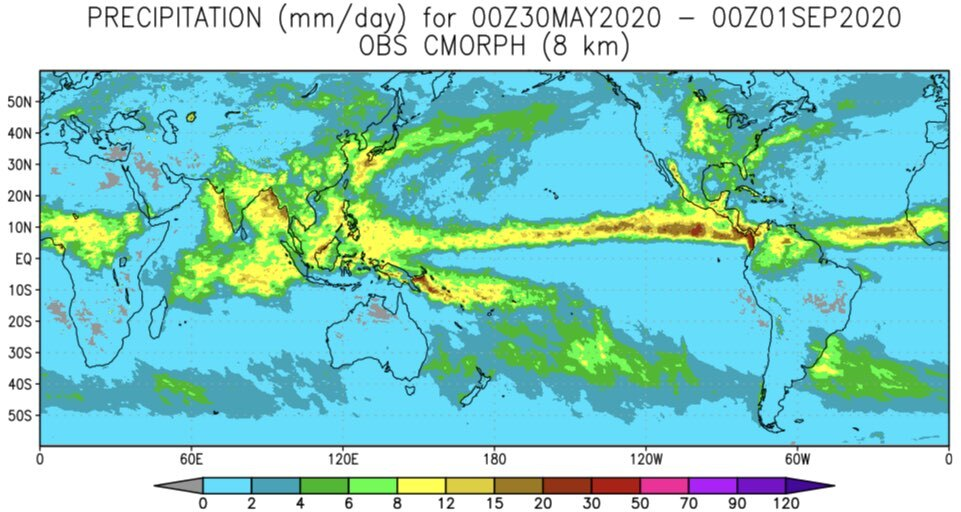
\includegraphics[width=0.375\textwidth]{./figs/cmorphjja.001_trim.jpeg}}
        \subfigure[BAM TQ0666L064]{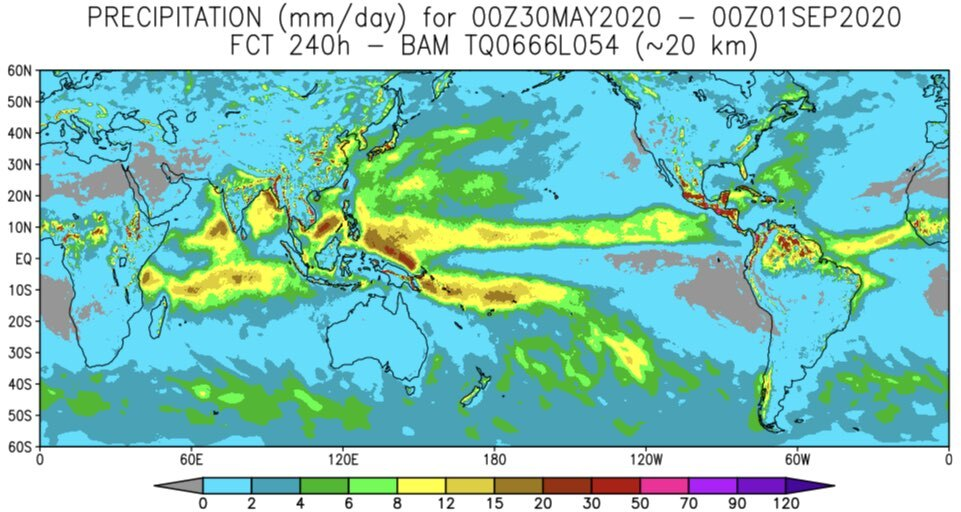
\includegraphics[width=0.375\textwidth]{./figs/bamjjafct240.001_trim.jpeg}}\\\vspace{-0.5em}
        \pause
        \subfigure[ENS MEAN MCGA TQ0126L028]{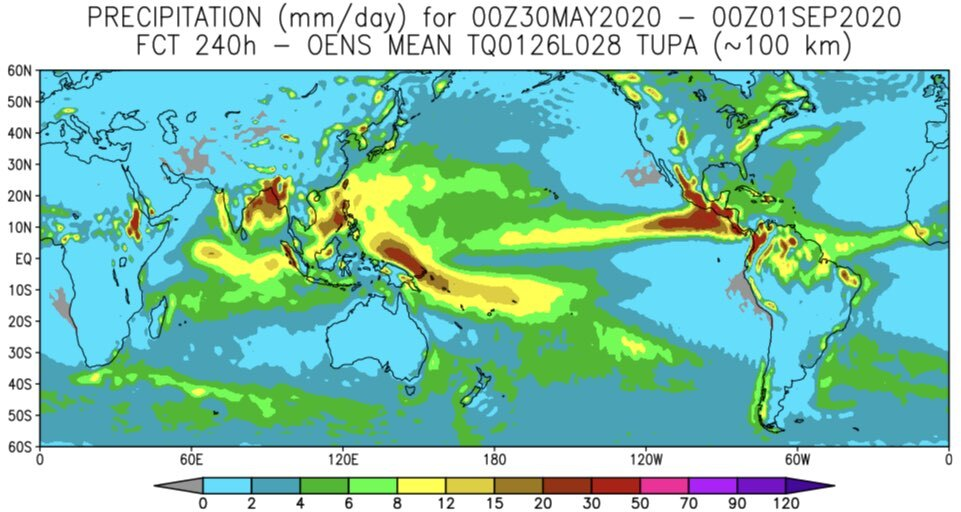
\includegraphics[width=0.375\textwidth]{./figs/smcmeanjjaxe6fct240.001_trim.jpeg}}
        \pause
        \subfigure[ENS MEAN BAM TQ0126L028]{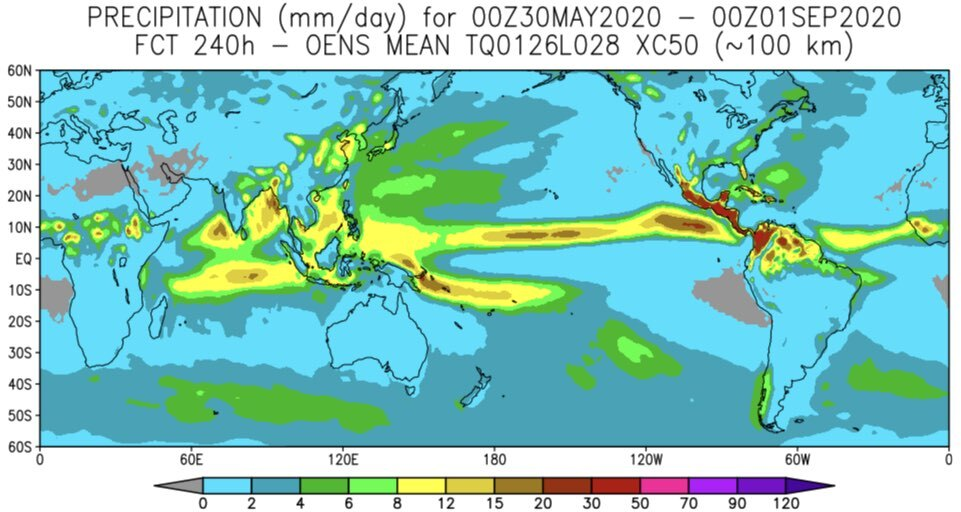
\includegraphics[width=0.375\textwidth]{./figs/smcmeanjjaxc50fct240.001_trim.jpeg}}
        \caption{}
    %\end{center}
\end{figure}
\end{frame}

\subsection{Skill e Espalhamento}

\begin{frame}{Estado Atual}
	\framesubtitle{Skill e Espalhamento}
	%\vspace{-1em}
\begin{figure}[H]
    %\begin{center}
    \centering
        \subfigure[Correlação de Anomalia]{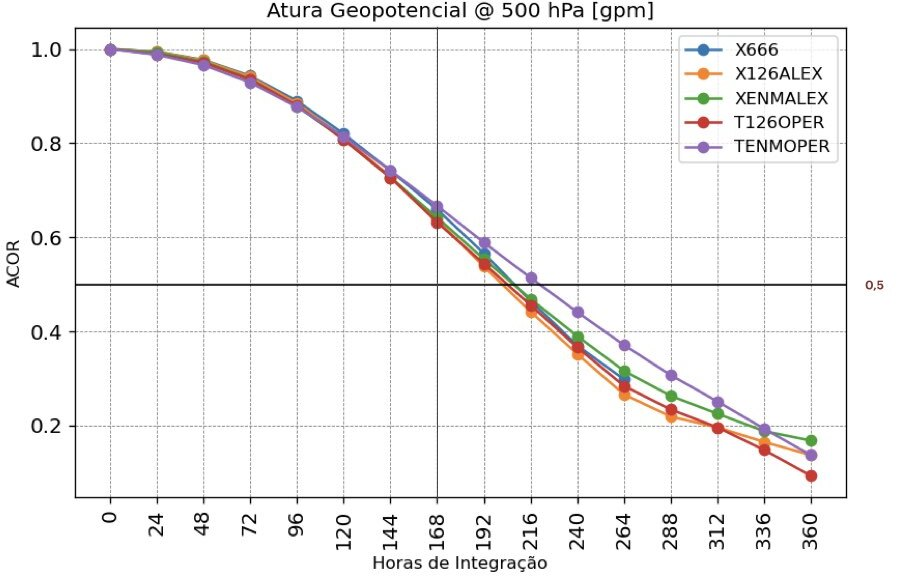
\includegraphics[width=0.48\textwidth]{./figs/Untitled.005_trim.jpeg}}
        \pause
        \subfigure[Espalhamento X REQM]{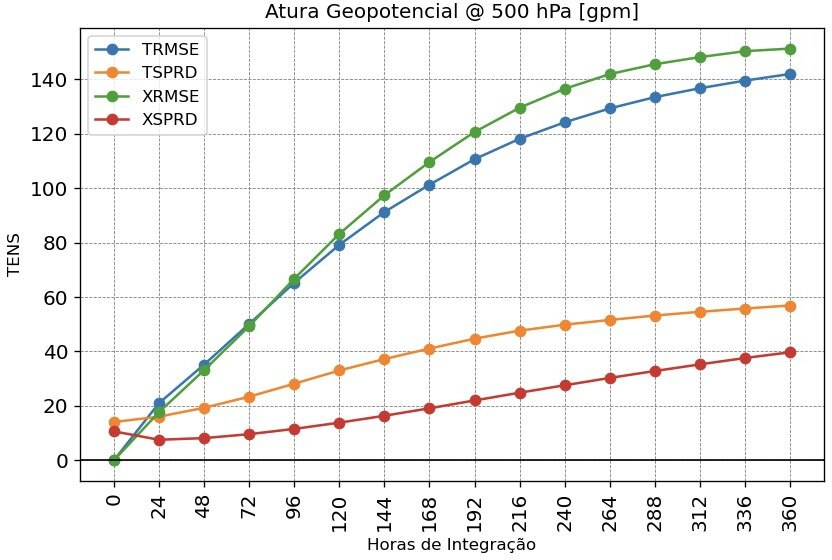
\includegraphics[width=0.48\textwidth]{./figs/Untitled.007_trim.jpeg}}
        \caption{}
    %\end{center}
\end{figure}
\end{frame}

\section{Planos Futuros}

\subsection{Método de Perturbação MB09}

% \begin{frame}{Planos Futuros}
% \framesubtitle{Método de Perturbação MB09}
% \vspace{-1em}
% \begin{figure}[t]
%   \centering
%   \includestandalone[width=0.75\linewidth]{./diagrama3}
% \end{figure}
% \end{frame}
%
%\subsection{Assimilação 3DEnVar}
%
%\begin{frame}{Planos Futuros}
%\framesubtitle{Assimilação 3DEnVar}
%\vspace{-0.75em}
%\begin{figure}[t]
%  \centering
%  \includestandalone[width=0.75\linewidth]{./diagrama1}
%\end{figure}
%\end{frame}
%
%\subsection{Assimilação 3DEnVar+MB09}
%
%\begin{frame}{Planos Futuros}
%\framesubtitle{Assimilação 3DEnVar+MB09}
%\vspace{-0.75em}
%\begin{figure}[t]
%  \centering
%  \includestandalone[width=0.75\linewidth]{./diagrama2}
%\end{figure}
%\end{frame}

 \begin{frame}{Planos Futuros}
 \framesubtitle{Método de Perturbação MB09}
\vspace{-1.5em}
\centering
\begin{tikzpicture}[node distance=2.25cm, thick,scale=1, every node/.style={scale=0.5}]

% Formas (col1)
\node (anl_ctr_ncep) [process1, visible on=<1->]                        
	{\begin{varwidth}{3cm}\Centering Condição Inicial\\Controle\\(NCEP) \end{varwidth}};
\node (anl_rdp_num1) [process2, below of=anl_ctr_ncep, visible on=<2->] 
	{\begin{varwidth}{3cm}\Centering Condição Inicial\\Pert. Rand. \#1 \end{varwidth}};
\node (anl_rdp_num2) [process3, below of=anl_rdp_num1, visible on=<2->] 
	{\begin{varwidth}{3cm}\Centering Condição Inicial\\Pert. Rand. \#2 \end{varwidth}};
\node (anl_rdp_dots) [process4, below of=anl_rdp_num2, visible on=<2->] 
	{\begin{varwidth}{3cm}\Centering \cdots \end{varwidth}};
\node (anl_rdp_numn) [process5, below of=anl_rdp_dots, visible on=<2->] 
	{\begin{varwidth}{3cm}\Centering Condição Inicial\\Pert. Rand. \#$n$ \end{varwidth}};

% Formas (col2)
\node (fct_ctr_ncep) [process1, xshift=4.75cm, visible on=<3->]            
	{\begin{varwidth}{3cm}\Centering Previsões\\Controle\\(48h, 3/3h) \end{varwidth}};
\node (fct_rdp_num1) [process2, below of=fct_ctr_ncep, visible on=<4->] 
	{\begin{varwidth}{3cm}\Centering Previsões Pert.\\Rand. \#1\\(48h, 3/3h) \end{varwidth}};
\node (fct_rdp_num2) [process3, below of=fct_rdp_num1, visible on=<4->] 
	{\begin{varwidth}{3cm}\Centering Previsões Pert.\\Rand. \#2\\(48h, 3/3h) \end{varwidth}};
\node (fct_rdp_dots) [process4, below of=fct_rdp_num2, visible on=<4->] 
	{\begin{varwidth}{3cm}\Centering \cdots \end{varwidth}};
\node (fct_rdp_numn) [process5, below of=fct_rdp_dots, visible on=<4->] 
	{\begin{varwidth}{3cm}\Centering Previsões Pert.\\Rand. \#$n$\\(48h, 3/3h) \end{varwidth}};

% Formas (col3)
\node (pert_eof1) [process2, xshift=9.5cm, yshift=-1.15cm, visible on=<6->] 
	{\begin{varwidth}{3cm}\Centering Perturbações EOF \#1 \end{varwidth}};
\node (pert_eof_dots) [process4, below of=pert_eof1, yshift=-1.15cm, visible on=<7->]    
	{\begin{varwidth}{3cm}\Centering \cdots \end{varwidth}};
\node (pert_eofn) [process5, below of=pert_eof_dots, yshift=-1.15cm, visible on=<8->]    
	{\begin{varwidth}{3cm}\Centering Perturbações EOF \#$n$ \end{varwidth}};

% Formas (col4)
\node (anl_ctr_ncep2) [process1, xshift=14cm, yshift=2.095cm, visible on=<11->] 
	{\begin{varwidth}{3cm}\Centering Condição Inicial\\Controle\\(NCEP) \#1 \end{varwidth}};

\node (pert_eof1_som) [process2, below of=anl_ctr_ncep2, visible on=<9->]     
	{\begin{varwidth}{3cm}\Centering Condição Inicial\\EOF \#1\\(Somada) \end{varwidth}};
\node (pert_eof1_sub) [process2, below of=pert_eof1_som, yshift=0.25cm, visible on=<9->]      
	{\begin{varwidth}{3cm}\Centering Condição Inicial\\EOF \#1\\(Subtraída) \end{varwidth}};
	
\node (pert_eof2_som) [process4, below of=pert_eof1_sub, yshift=0.9cm, visible on=<10->]      
	{\begin{varwidth}{3cm}\Centering \cdots \end{varwidth}};
\node (pert_eof2_sub) [process4, below of=pert_eof2_som, yshift=0.15cm, visible on=<10->]      
	{\begin{varwidth}{3cm}\Centering \cdots \end{varwidth}};
	
\node (pert_eofn_som) [process5, below of=pert_eof2_sub, yshift=0.9cm, visible on=<11->]      
	{\begin{varwidth}{3cm}\Centering Condição Inicial\\EOF \#$n$\\(Somada) \end{varwidth}};
\node (pert_eofn_sub) [process5, below of=pert_eofn_som, yshift=0.25cm, visible on=<11->]      
	{\begin{varwidth}{3cm}\Centering Condição Inicial\\EOF \#$n$\\(Subtraída) \end{varwidth}};

% Formas (col5)
\node (fct_ctr_ncep2) [process1, xshift=18.5cm, yshift=2.095cm, visible on=<13->] 
	{\begin{varwidth}{3cm}\Centering Previsão\\Membro \#1\\(360h, 6/6h) \#1 \end{varwidth}};
	
\node (fct_eof1_som) [process2, below of=fct_ctr_ncep2, visible on=<13->]       
	{\begin{varwidth}{3cm}\Centering Previsão\\Membro \#2\\(360h, 6/6h) \end{varwidth}};
\node (fct_eof1_sub) [process2, below of=fct_eof1_som, yshift=0.25cm, visible on=<13->]        
	{\begin{varwidth}{3cm}\Centering Previsão Membro \#3\\(360h, 6/6h) \end{varwidth}};
	
\node (fct_eof2_som) [process4, below of=fct_eof1_sub, yshift=0.9cm, visible on=<13->]        
	{\begin{varwidth}{3cm}\Centering \cdots \end{varwidth}};
\node (fct_eof2_sub) [process4, below of=fct_eof2_som, yshift=0.15cm, visible on=<13->]        
	{\begin{varwidth}{3cm}\Centering \cdots \end{varwidth}};
	
\node (fct_eofn_som) [process5, below of=fct_eof2_sub, yshift=0.9cm, visible on=<13->]        
	{\begin{varwidth}{3cm}\Centering Previsão\\Membro \#$n-1$\\(360h, 6/6h) \end{varwidth}};
\node (fct_eofn_sub) [process5, below of=fct_eofn_som, yshift=0.25cm, visible on=<13->]     
	{\begin{varwidth}{3cm}\Centering Previsão\\Membro \#$n$\\(360h, 6/6h) \end{varwidth}};

% Flechas (col1)
\draw [arrow, visible on=<2->] (anl_ctr_ncep) -- node[anchor=west] {(RAND)} (anl_rdp_num1);
\draw [arrow, dashed, visible on=<2->] (anl_rdp_num1) -- node[anchor=west] {(RAND)} (anl_rdp_num2);
\draw [arrow, dashed, visible on=<2->] (anl_rdp_num2) -- node[anchor=west] {(RAND)} (anl_rdp_dots);
\draw [arrow, dashed, visible on=<2->] (anl_rdp_dots) -- node[anchor=west] {(RAND)} (anl_rdp_numn);

% Flechas (col2)
\draw [stealth-stealth, visible on=<5->] (fct_ctr_ncep) -- node[anchor=west] {(EOF)} (fct_rdp_num1);
\draw [arrow, dashed, visible on=<5->] (fct_rdp_num1) -- node[anchor=west] {(EOF)} (fct_rdp_num2);
\draw [arrow, dashed, visible on=<5->] (fct_rdp_num2) -- node[anchor=west] {(EOF)} (fct_rdp_dots);
\draw [arrow, dashed, visible on=<5->] (fct_rdp_dots) -- node[anchor=west] {(EOF)} (fct_rdp_numn);

% Flechas (col1->col2)
\draw [arrow, visible on=<3->] (anl_ctr_ncep) -- (fct_ctr_ncep);
\draw [arrow, visible on=<4->] (anl_rdp_num1) -- (fct_rdp_num1);
\draw [arrow, visible on=<4->] (anl_rdp_num2) -- (fct_rdp_num2);
\draw [arrow, visible on=<4->] (anl_rdp_dots) -- (fct_rdp_dots);
\draw [arrow, visible on=<4->] (anl_rdp_numn) -- (fct_rdp_numn);

% Linhas e flechas entre col2 e col3
\node [coordinate, right = 0.4375cm of fct_ctr_ncep] (ADL1){};
\draw [arrow, visible on=<6->] (fct_ctr_ncep) -- (ADL1) |- (pert_eof1);

\node [coordinate, right = 0.4375cm of fct_rdp_num1] (ADL2){};
\draw [arrow, visible on=<6->] (fct_rdp_num1) -- (ADL2) |- (pert_eof1);

\node [coordinate, right = 0.4375cm of fct_ctr_ncep] (ADL3){};
\draw [arrow, visible on=<7->] (fct_ctr_ncep) -- (ADL3) |- (pert_eof_dots);

\node [coordinate, right = 0.4375cm of fct_rdp_dots] (ADL4){};
\draw [arrow, visible on=<7->] (fct_rdp_dots) -- (ADL4) |- (pert_eof_dots);

\node [coordinate, right = 0.4375cm of fct_ctr_ncep] (ADL5){};
\draw [arrow, visible on=<8->] (fct_ctr_ncep) -- (ADL5) |- (pert_eofn);

\node [coordinate, right = 0.4375cm of fct_rdp_numn] (ADL6){};
\draw [arrow, visible on=<8->] (fct_rdp_numn) -- (ADL6) |- (pert_eofn);

% Linhas e flechas entre col3 e col4 e entre as colunas col4 e col5
\node [coordinate, right = 0.4375cm of pert_eof1] (BDL1){};
\draw [arrow, visible on=<9->] (pert_eof1) -- (BDL1) |- (pert_eof1_som);

\node [coordinate, right = 0.4375cm of pert_eof1] (BDL2){};
\draw [arrow, visible on=<9->] (pert_eof1) -- (BDL2) |- (pert_eof1_sub);

\node [coordinate, right = 0.4375cm of pert_eof_dots] (BDL3){};
\draw [arrow, visible on=<10->] (pert_eof_dots) -- (BDL3) |- (pert_eof2_som);

\node [coordinate, right = 0.4375cm of pert_eof_dots] (BDL4){};
\draw [arrow, visible on=<10->] (pert_eof_dots) -- (BDL4) |- (pert_eof2_sub);

\node [coordinate, right = 0.4375cm of pert_eofn] (BDL5){};
\draw [arrow, visible on=<11->] (pert_eofn) -- (BDL5) |- (pert_eofn_som);

\node [coordinate, right = 0.4375cm of pert_eofn] (BDL6){};
\draw [arrow, visible on=<11->] (pert_eofn) -- (BDL6) |- (pert_eofn_sub);

% Flechas (col4->col5)
\draw [arrow, visible on=<13->] (anl_ctr_ncep2) -- (fct_ctr_ncep2);
\draw [arrow, visible on=<13->] (pert_eof1_som) -- (fct_eof1_som);
\draw [arrow, visible on=<13->] (pert_eof1_sub) -- (fct_eof1_sub);
\draw [arrow, visible on=<13->] (pert_eof2_som) -- (fct_eof2_som);
\draw [arrow, visible on=<13->] (pert_eof2_sub) -- (fct_eof2_sub);
\draw [arrow, visible on=<13->] (pert_eofn_som) -- (fct_eofn_som);
\draw [arrow, visible on=<13->] (pert_eofn_sub) -- (fct_eofn_sub);

% Linhas e flechas entre col1 e col4
\node [coordinate, above = 0.655cm of anl_ctr_ncep] (EDL1){};
\draw [path, visible on=<11->] (anl_ctr_ncep) |- (anl_ctr_ncep2);

% Retângulos das colunas 4 e 5
%\draw[pattern=north west lines, pattern color=blue, thick, dotted] ($(anl_ctr_ncep2.north west)+(-0.5,0.25)$)  rectangle ($(pert_eofn_sub.south east)+(0.3,-1)$);
\draw[thick, dotted, visible on=<12->] ($(anl_ctr_ncep2.north west)+(-0.5,0.25)$)  rectangle ($(pert_eofn_sub.south east)+(0.3,-1)$);
\node (r1Label)[below=0.15cm of pert_eofn_sub, visible on=<12->] {\begin{varwidth}{3cm}\Centering \textit{Ensemble} final\\de Análises\\Tamanho: $2n+1$ \end{varwidth}};

\draw[thick, dotted, visible on=<14->] ($(fct_ctr_ncep2.north west)+(-0.5,0.25)$)  rectangle ($(fct_eofn_sub.south east)+(0.3,-1)$);
\node (r1Label)[below=0.15cm of fct_eofn_sub, visible on=<14->] {\begin{varwidth}{3cm}\Centering \textit{Ensemble} final\\de Previsões\\Tamanho: $2n+1$ \end{varwidth}};

\end{tikzpicture}

 \end{frame}

 \begin{frame}{Planos Futuros}
 \framesubtitle{Método de Perturbação MB09}
% \vspace{-1em}

 \end{frame}
 
  \begin{frame}{Planos Futuros}
 \framesubtitle{Método de Perturbação MB09}
% \vspace{-1em}

 \end{frame}

\begin{frame}{Assimilação 3DEnVar+MB09}
\framesubtitle{Um Monte de Membros}
\begin{block}{Juntando tudo:}
	\begin{itemize}
		\item Combinação entre as técnicas EnKF e MB09;
		\pause
		\item Vantagem: possibilidade de usar a mesma análise atmosférica para produzir o ensemble usando o framework da assimilação (i.e., 3DEnVar);
		\pause
		\item Este exercício servirá para testar as técnicas para serem aplicadas ao MONAN;
		\pause
		\item O ensemble do 3DEnVar (laranja) parece ser diferente do ensemble gerado pelo MB09 (rosa e azul).
	\end{itemize}
\end{block}
\pause
\begin{block}{Então...}
	\begin{itemize}
		\item O EnKF fornece características que complementam aquelas geradas pela e EOF? 
		\item A análise determinística do 3DEnVar é um bom substituto para a análise do NCEP?
	\end{itemize}
\end{block}
\end{frame}

\begin{frame}{Assimilação 3DEnVar+MB09}
\framesubtitle{Um Monte de Membros}
%\vspace{-2em}
	\begin{columns}[t]
    	\begin{column}{.5\textwidth}
   		    %\vspace{1em}
    		\begin{itemize}
        		\item Ponto sobre São Paulo (46S;23W);
        		\item Previsão da PSNM 15 dias;
        		\item Válido para 2012122000-2013010400.
    		\end{itemize}
    		\vspace{1em}
    		\begin{itemize}
				\item O EnKF fornece características que complementam aquelas geradas pela e EOF? 
				\item A análise determinística do 3DEnVar é um bom substituto para a análise do NCEP?
			\end{itemize}
        \end{column}
        \begin{column}{.5\textwidth}
            \vspace{-3em}
			\begin{figure}[t]
			  \centering
			  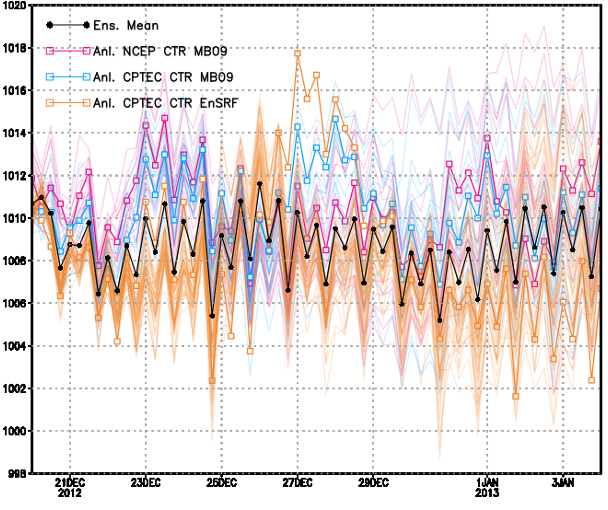
\includegraphics[width=1.\linewidth]{./figs/spaguete71.png}
			\end{figure}
        \end{column}
    \end{columns}
\end{frame}

\begin{frame}{Assimilação 3DEnVar+MB09}
\framesubtitle{Análises 3DEnVar e NCEP para o oensMB09}
%\vspace{-2em}
	\begin{columns}[t]
	    \vspace{2em}
    	\begin{column}{.45\textwidth}
    		\centering
    		Prevsisão de prec. a partir das análises do NCEP e 3DEnVar
        	\begin{figure}[t]
       	   	    %\vspace{3em}
				\centering
				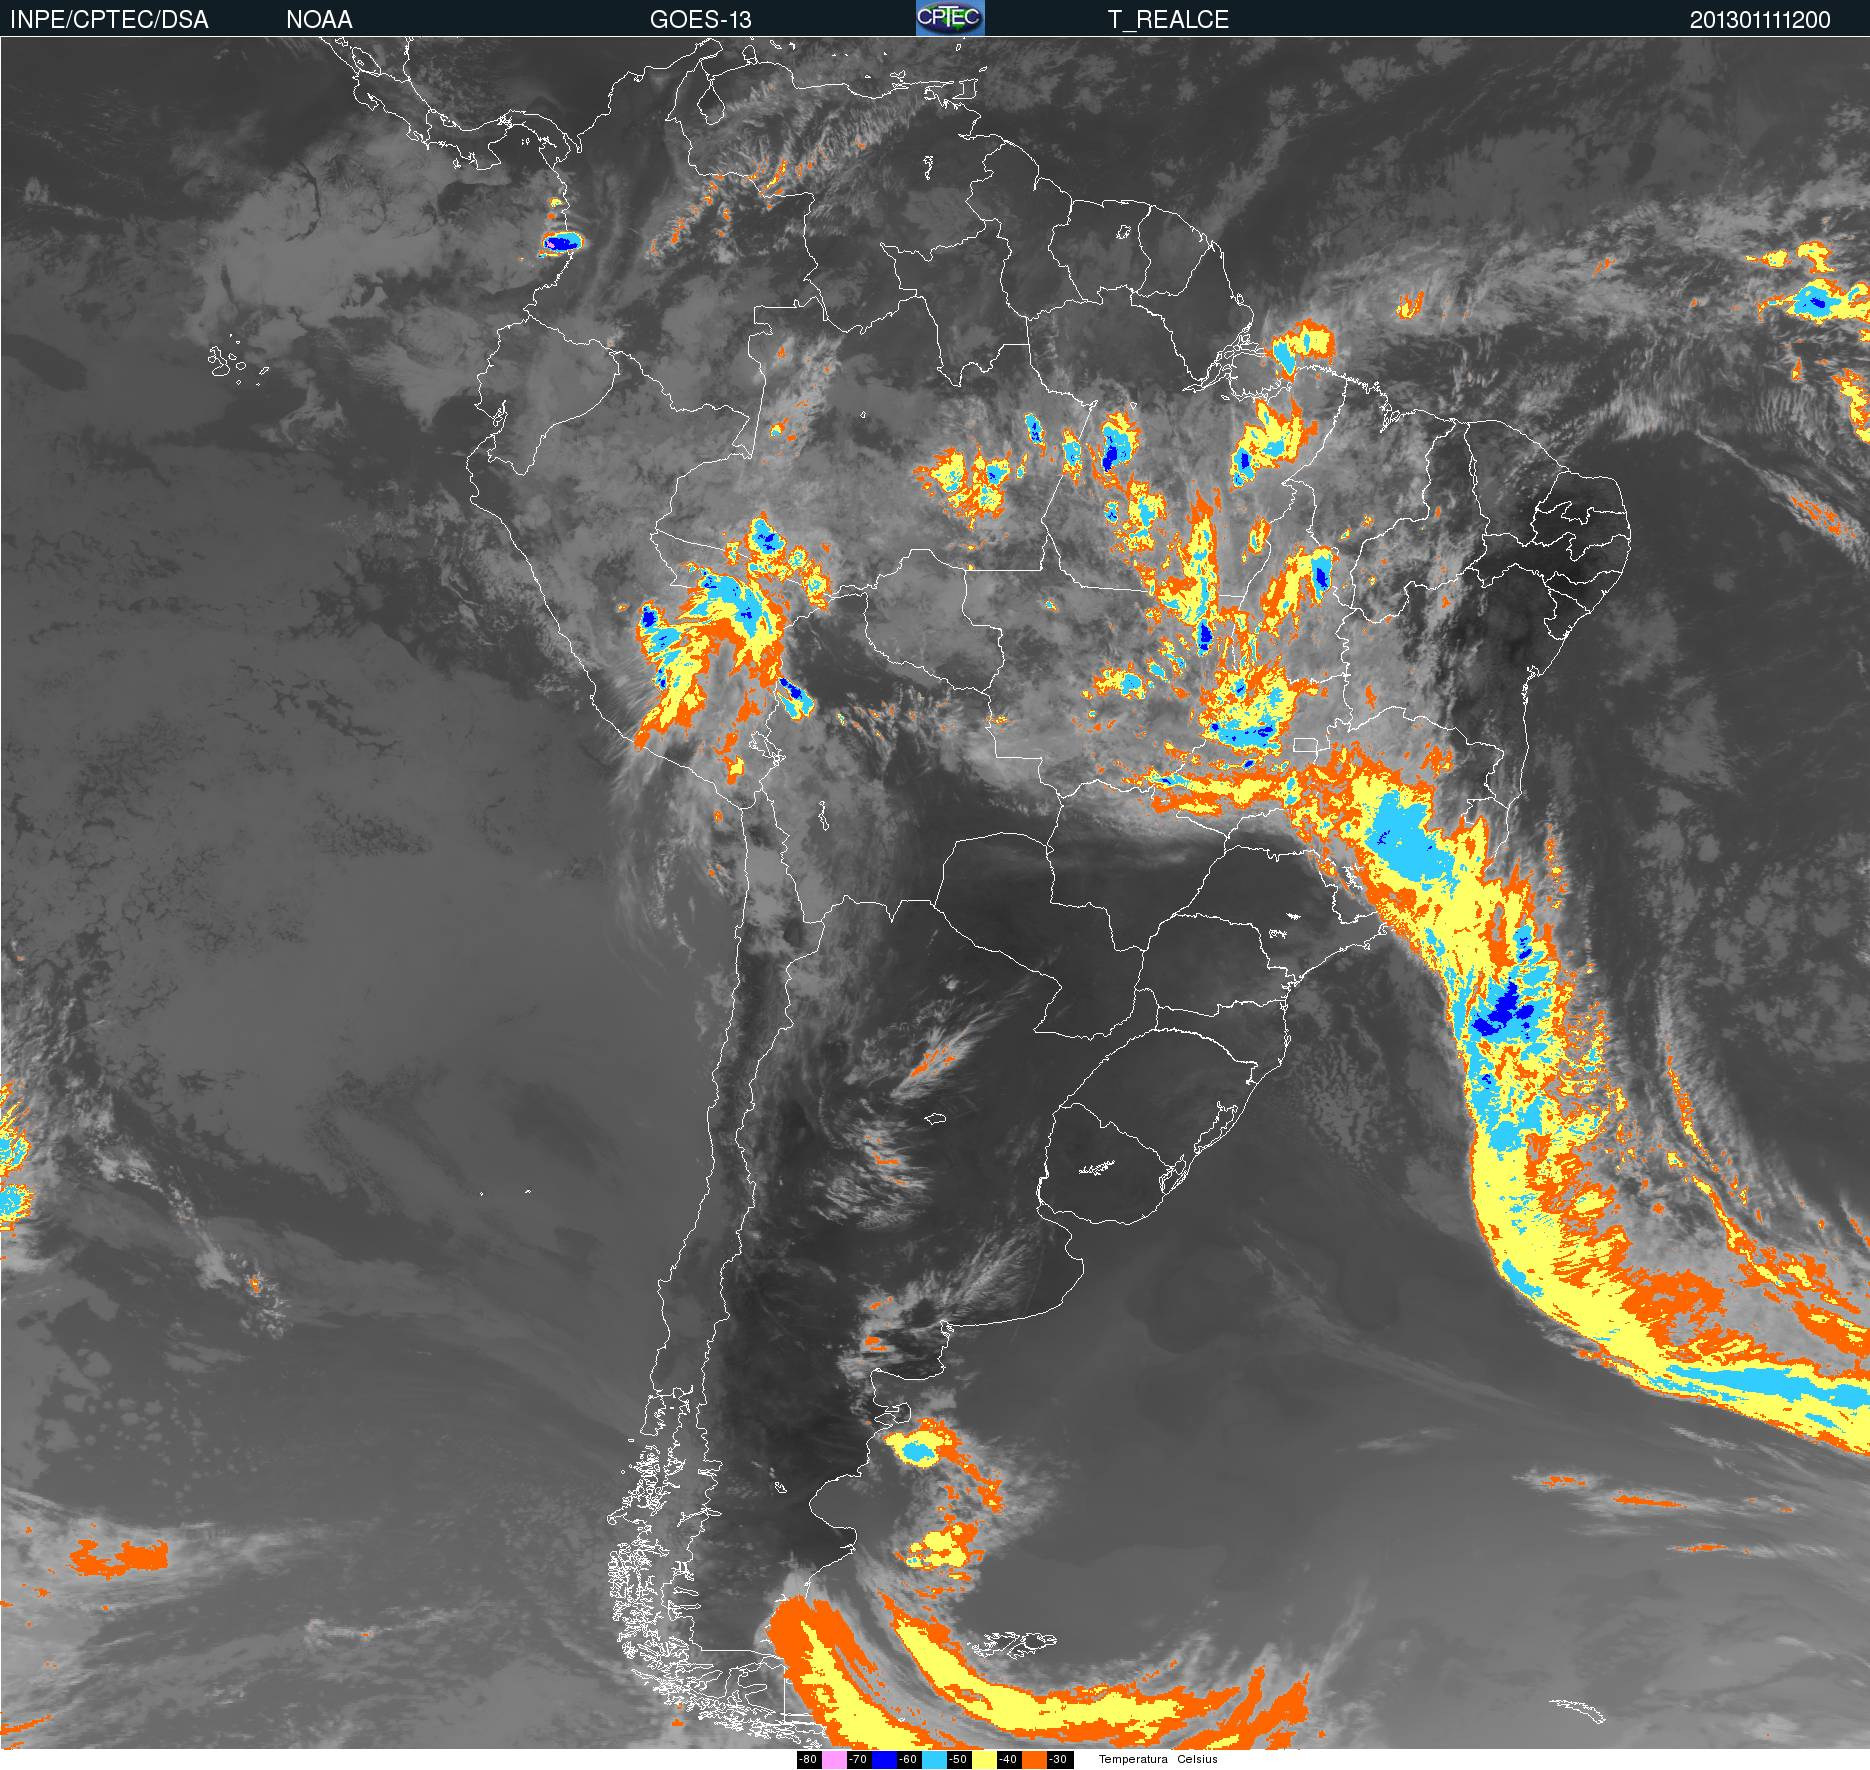
\includegraphics[width=0.8\linewidth]{./figs/goes13.jpg}
				\caption{GOES 13 IR (11 Jan 2013, 12Z)}
			\end{figure}
        \end{column}
        \begin{column}{.5\textwidth}
        	\begin{figure}[H]
        		\vspace{-2em}
				%\begin{center}
				\centering
        			\subfigure[CTR NCEP]{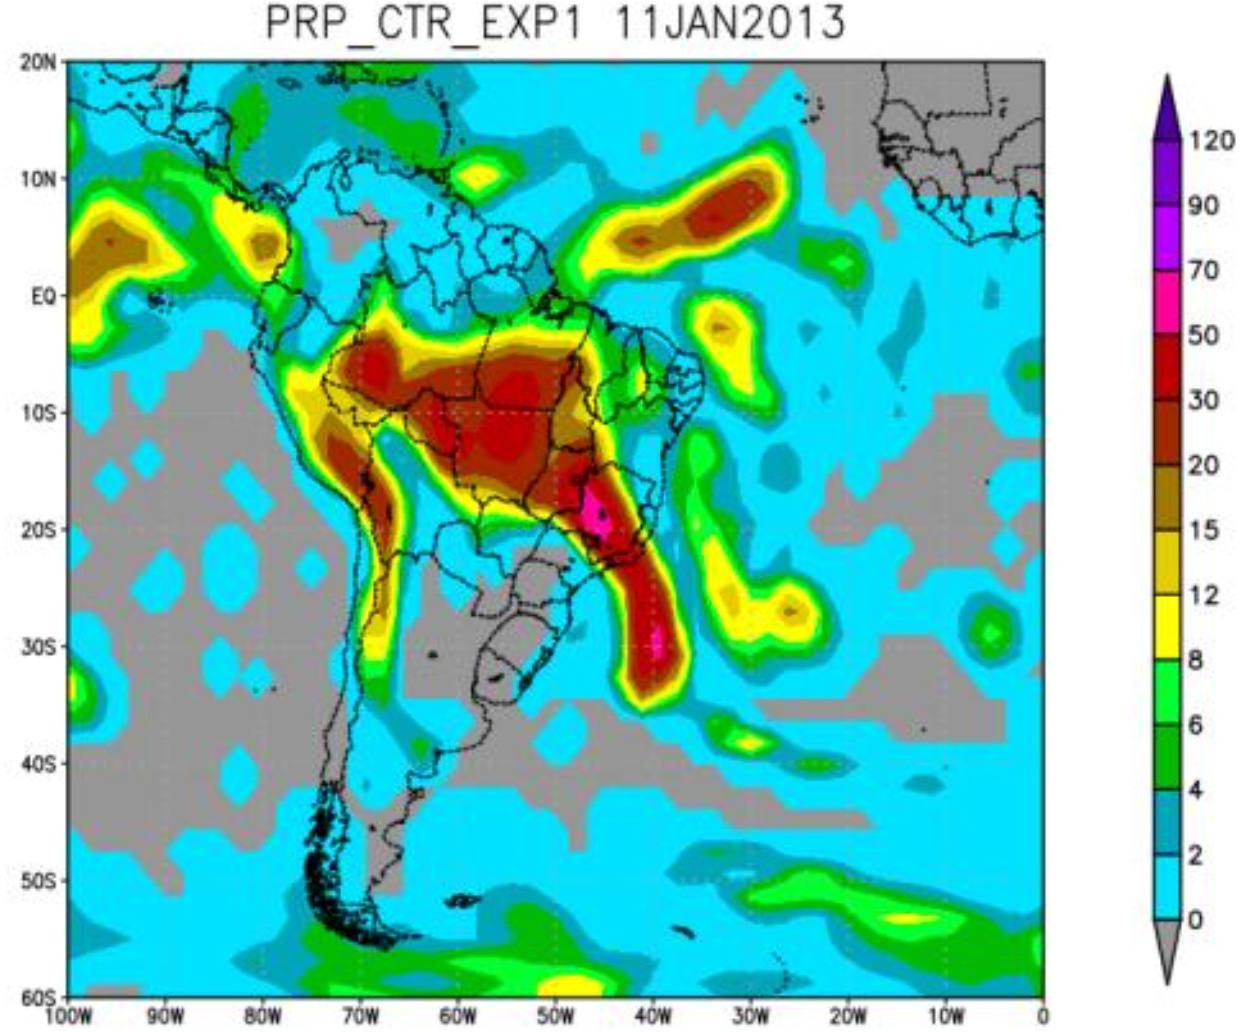
\includegraphics[width=0.45\textwidth]{./figs/prec_ctr_exp1_trim.jpg}}
        			\subfigure[MEAN NCEP]{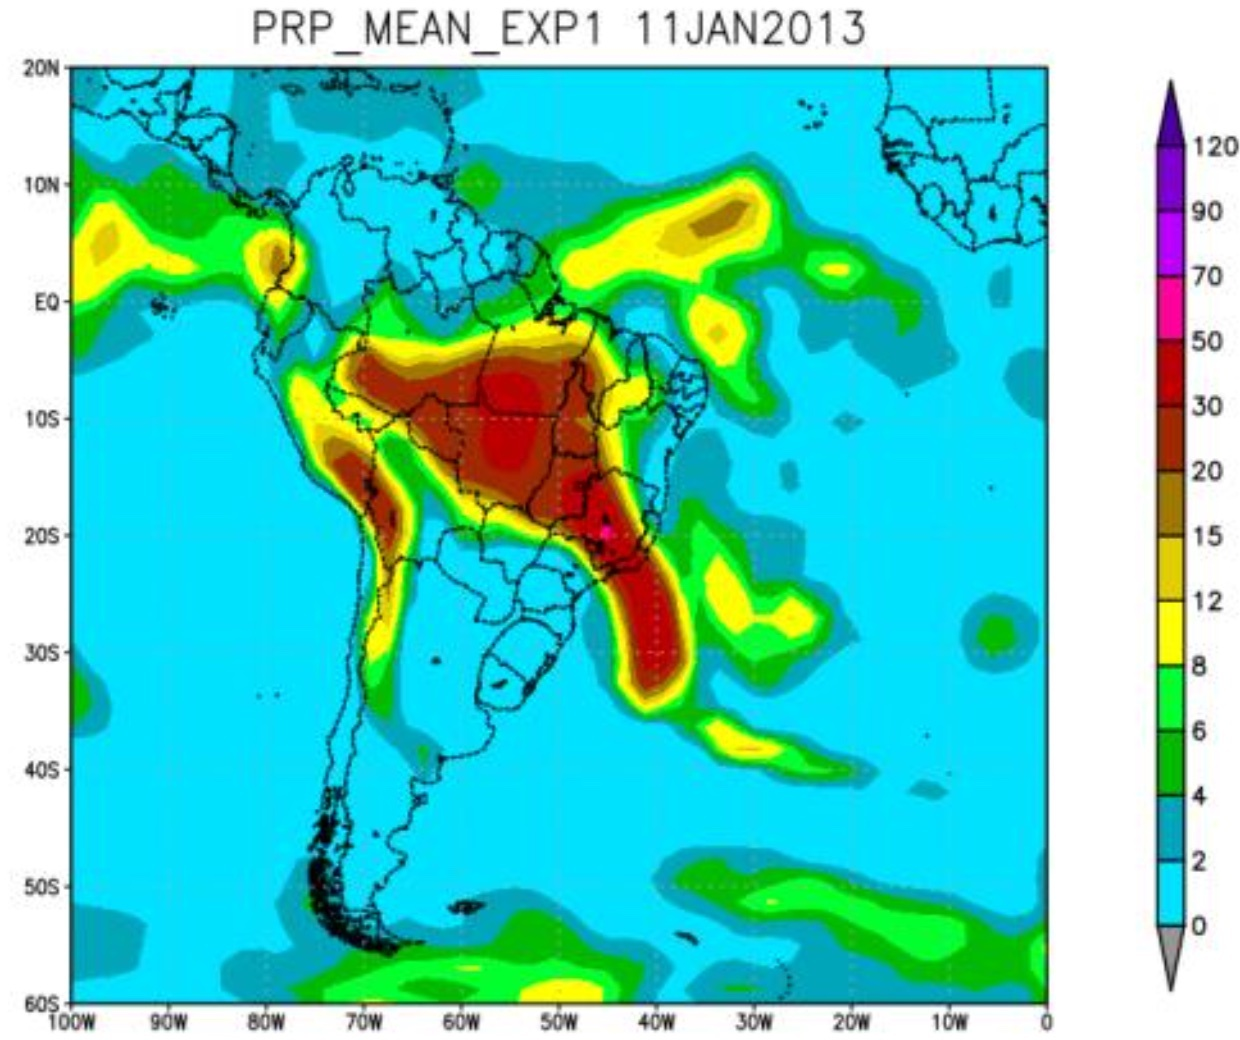
\includegraphics[width=0.45\textwidth]{./figs/prec_mean_exp1_trim.jpg}}\\
        			\pause
        			\subfigure[CTR 3DEnVar]{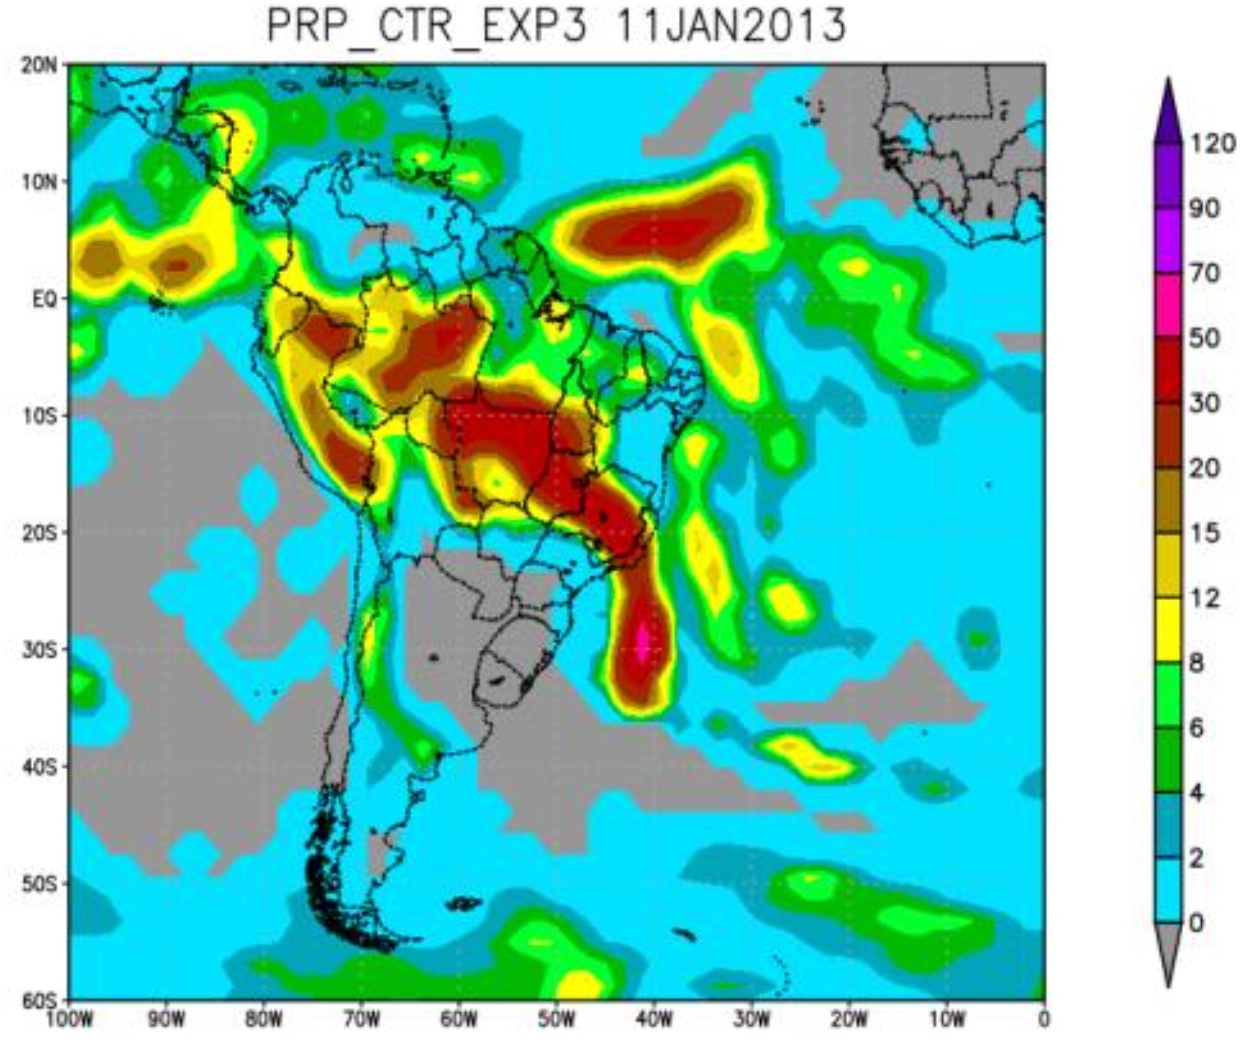
\includegraphics[width=0.45\textwidth]{./figs/prec_ctr_exp3_trim.jpg}}
        			\pause
        			\subfigure[MEAN 3DEnVar]{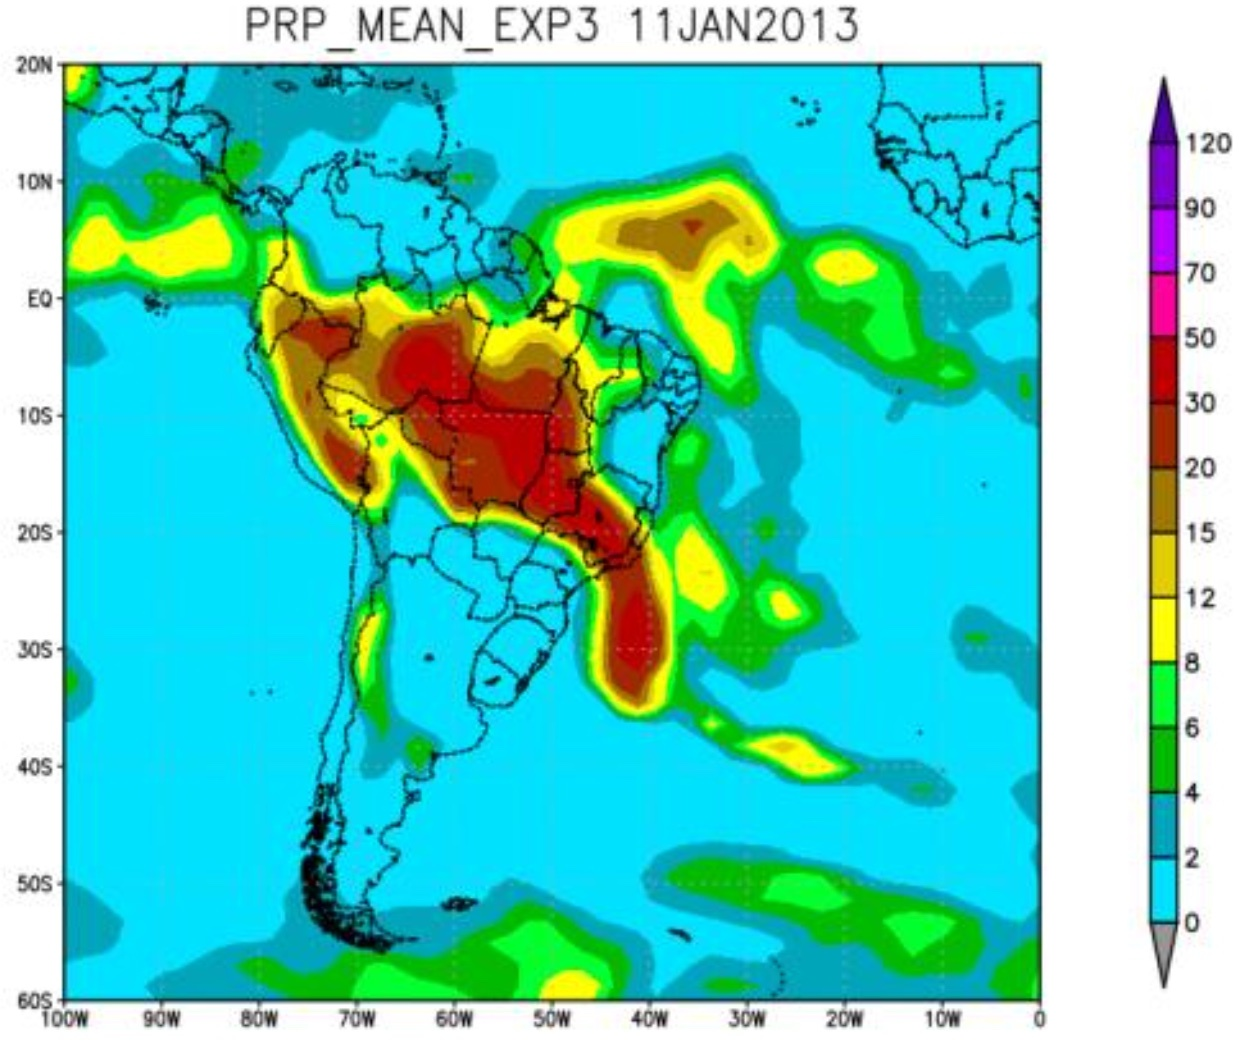
\includegraphics[width=0.45\textwidth]{./figs/prec_mean_exp3_trim.jpg}}
    			%\end{center}
			\end{figure}
        \end{column}
    \end{columns}
\end{frame}

\section{Dificuldades e Desafios}

\begin{frame}{Dificuldades e Desafios}
\framesubtitle{Algumas Questões \faQuestionCircle}
	\begin{itemize}
		\item Controlar o espalhamento do ensemble das análises e previsões;
		\pause
		\item Lidar com o custo computacional elevado:
		\begin{itemize}
			\item Inteligência artificial é um caminho: uma rede neural pode emular o EnKF no 3DEnVar?
		\end{itemize}
		\pause
		\item Finalidade do ensemble (aplicação): ter maior resolução ou ter conjunto maior?
		\item Com um centro do nosso tamanho, com as dificuldades que temos, precisamos enxugar as nossas suítes:
		\begin{itemize}
			\item Assimilação 3DEnVar: assimilação + PNT det. + PNT por conjunto (tempo estendido e subsazonal), utilizando a mesma versão do modelo (com configurações adequadas para cada aplicação).
		\end{itemize}
	\end{itemize}
\end{frame}

\begin{frame}
\frametitle{Referências Bibliográficas}
\framesubtitle{\faBookOpen~\faNewspaper[regular]~\faIcon[regular]{file}}
\vspace{-1em}
\bibliography{referencias}
\end{frame}

% Frame Final (NÃO MODIFICAR)
\usebackgroundtemplate%
{%
	
\includegraphics[width=\paperwidth,height=\paperheight]{fundo_slide_inpe_sem_logo.png}%	
}

\begingroup
\setbeamertemplate{footline}{}
{\nologo
\begin{frame}
	\begin{figure}[H]
    	\vspace{-4em}
		%\begin{center}
		\centering
        	\hspace*{1.5em}
\includegraphics[width=1.\textwidth]{DesinacaoNominativaCentralizada2020.pdf}
    	%\end{center}
	\end{figure}
\end{frame}
}
\endgroup

\end{document}
